\documentclass{UTNetLab}

\title{A Single Segment Network}
\newcommand\reference{
   S. Panwar, S. Mao, J.-dong Ryoo, and Y. Li, “A single segment network,” in TCP/IP Essentials: A Lab-Based Approach, Cambridge: Cambridge University Press, 2004, pp. 43–60.
}

\begin{document}
	 
	 \section*{Objectives}
	 \begin{itemize}
	 	\item Network interfaces and interface configuration.
	 	\item Network load and statistics.
	 	\item The Address Resolution Protocol (ARP) and its operations.
	 	\item ICMP messages and Ping.
	 	\item Concept of subnetting.
	 	\item Duplicate IP addresses and incorrect subnet masks.
	 \end{itemize}
 
	\part{Network Interface Exercises}
	The following exercises use the single segment network topology shown in \hyperref[fig:1.3]{Figure~1.3}.
	\begin{center}
		\begin{minipage}{0.48\textwidth}
			\begin{flushleft}
				\begin{table}[H]
					\caption{The IP addresses of the hosts (Table~1.2)}
					\centering
					\begin{tabular}{ c c c }
						\hline \hline
						Host & IP Address & Subnet Mask \\
						\hline 
						h0 & 128.238.66.100 & 255.255.255.0 \\
						h1 & 128.238.66.101 & 255.255.255.0 \\
						h2 & 128.238.66.102 & 255.255.255.0 \\
						h3 & 128.238.66.103 & 255.255.255.0 \\
						h4 & 128.238.66.104 & 255.255.255.0 \\
						h5 & 128.238.66.105 & 255.255.255.0 \\
						h6 & 128.238.66.106 & 255.255.255.0 \\
						h7 & 128.238.66.107 & 255.255.255.0 \\
						\hline \hline
					\end{tabular}
				\end{table}
			\end{flushleft}
		\end{minipage}
		\begin{minipage}{0.48\textwidth}
			\begin{flushright}
				\begin{figure}[H]
					\centering
					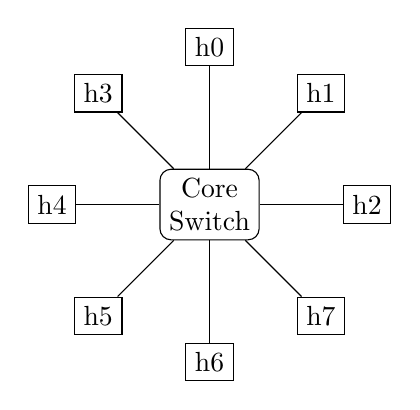
\begin{tikzpicture}
						\node[draw,align=center,rounded corners] (s) at (0,0){Core\\Switch};
						\node[draw] (h0) at (0,2){h0};
						\node[draw] (h1) at ({sqrt(2)},{sqrt(2)}){h1};
						\node[draw] (h2) at (2,0){h2};
						\node[draw] (h3) at (-{sqrt(2)},{sqrt(2)}){h3};
						\node[draw] (h4) at (-2,0){h4};
						\node[draw] (h5) at (-{sqrt(2)},-{sqrt(2)}){h5};
						\node[draw] (h6) at (0,-2){h6};
						\node[draw] (h7) at ({sqrt(2)},-{sqrt(2)}){h7};
						
						\draw (h0) -- (s);
						\draw (h1) -- (s);
						\draw (h2) -- (s);
						\draw (h3) -- (s);
						\draw (h4) -- (s);
						\draw (h5) -- (s);
						\draw (h6) -- (s);
						\draw (h7) -- (s);
					\end{tikzpicture}
					\caption{A single segment network (Figure~1.3)}\label{fig:1.3}
				\end{figure}
			\end{flushright}
		\end{minipage}
	\end{center}

\section{Network Interfaces}

    Use the following command
    
    \fcolorbox{blue}{red!10}{h\textsubscript{0}'s Console}
    \lstset{backgroundcolor=\color{red!10}}
    \begin{lstlisting}
    ifconfig -a
    \end{lstlisting}

    to display information about the network interfaces on \textit{h0}.
    Find the IP address and the net mask of your machine.
    
    \begin{report}
        \item How many interfaces does the host have?
            List all the interfaces found, give their names, and explain their functions briefly.

        \item What are the MTUs of the interfaces on \textit{h0}?

        \item Is network subnetted?
            What is the reasoning for your answer? What the experimental are the reasons for subnetting?
    \end{report}


\section{Local Host Dump}
    Run the following command on host \textit{h0} to capture loopback interface packets in the background

    \fcolorbox{blue}{blue!10}{h\textsubscript{0}'s Console}
    \lstset{backgroundcolor=\color{blue!10}}
    \begin{lstlisting}
    tcpdump -i lo &
    \end{lstlisting}

    While the \lstinline{tcpdump} command is running, run the following command

    \fcolorbox{blue}{red!10}{h\textsubscript{0}'s Console}
    \lstset{backgroundcolor=\color{red!10}}
    \begin{lstlisting}
    ping 127.0.0.1
    \end{lstlisting}

    To stop the \lstinline{ping} you can use \texttt{Ctrl + C} and to stop the background \lstinline{tcpdump} you can first run \lstinline{fg} command to bring it to the foreground and then use \texttt{Ctrl + C} to stop it.

    \begin{report}
        \item From the \lstinline{ping} output, is the 127.0.0.1 interface on?
            Can you see any ICMP message sent from your host in the \lstinline{tcpdump} output?
            Why?
    \end{report}


\section{Network Statistics}
    By using below command, collect the statistics from all the hosts on the network
    \footnote{You can use \lstinline{ifconfig} instead.}.
    
    \fcolorbox{blue}{red!10}{ {h\textsubscript{0}}'s Console }
    \lstset{backgroundcolor=\color{red!10}}
    \begin{lstlisting}
    netstat -ie
    \end{lstlisting}
    
    
    By using "\lstinline{netlab}" as login username and password, we can \lstinline{telnet} to other hosts and run the following command there.\footnote{%
    	After you are done with a remote host, you should exit the \lstinline{telnet} session before you \lstinline{telnet} to another remote host.
    	Recursive \lstinline{telnet} will generate unnecessary data in the \lstinline{tcpdump} output and cause confusion.
    }
    
    \fcolorbox{blue}{red!10}{ {h\textsubscript{0}}'s Console }
    \lstset{backgroundcolor=\color{red!10}}
    \begin{lstlisting}
    telnet 128.238.66.101
    //after login to h1
    netstat -ie
    \end{lstlisting}
    
    Save the \lstinline{netstat -ie} outputs.

    Note: If you don’t see a significant amount of output packets in the \lstinline{netstat} output, the machine was probably restarted recently.
    You may do this experiment later, or use the following \lstinline{socket} command to generate some network traffic:
    
    \fcolorbox{blue}{green!10}{ {h\textsubscript{0}}'s Console }
    \lstset{backgroundcolor=\color{green!10}}
    \begin{lstlisting}[emph={remote-host}]
    socket -u -i -n200 remote-host echo
    \end{lstlisting}
    You should replace \lstinline{remote-host} with valid IP address like 128.238.66.104
    
    \begin{report}
        \item Calculate the average collision rate over all the hosts for the set of statistics you collected in this exercise.
    \end{report}

\part{ARP Exercises}
    In the following experiment, we shall examine the host ARP table and the ARP operation, including two interesting cases: proxy ARP and gratuitous ARP.
    You may need to find \textbf{MAC} addresses of the host and router interfaces, and record these \textbf{MAC} addresses.
    You need these \textbf{MAC} addresses for the exercises and lab report (as table of host and \textbf{MAC}).

\section{ARP Table}
     use the following command to see the entire ARP table on \textit{h0}.  Observe that all the IP addresses displayed are on the same subnet.
    
    \fcolorbox{blue}{red!10}{ {h\textsubscript{0}}'s Console }
    \lstset{backgroundcolor=\color{red!10}}
    \begin{lstlisting}
    arp -a
    \end{lstlisting}
   
    If you find that all the remote hosts are in \textit{h0}’s ARP table, you need to delete a remote host from the table, using:
    \footnote{If you deleted \textit{h0}’s IP address from the ARP table by mistake, you must add the entry back in the table.
    See the \lstinline{arp} manual page to add.
    Note that, in order for \textit{h0} to reply to the ARP requests, the ARP entry of \textit{h0} must have the \lstinline{P} flag in the ARP table.}
    
    \fcolorbox{blue}{green!10}{ {h\textsubscript{0}}'s Console }
    \lstset{backgroundcolor=\color{green!10}}
    \begin{lstlisting}[emph={remote-host}]
    arp -d remote-host
    \end{lstlisting}

    Save the ARP table for your lab report.
    
    While \lstinline{wireshark} is running to capture traffic from your machine,
    
    \fcolorbox{blue}{lime!30}{ h\textsubscript{0}'s Wireshark} 
    \lstset{backgroundcolor=\color{lime!30}}
    \begin{lstlisting}
    Run wireshark on eth1
    \end{lstlisting}
    % and enable 'Ethernet headers' (MAC addresses) and disable 'Name Resolution' (IP-to-hostname) in Wireshark's settings
    \lstinline{ping} a remote host that has no entry in the \textit{ h0} ARP table by running the following command: (for example, we assume that  \textit{h4} has no entry in \textit{h0} ARP table)
    
 \fcolorbox{blue}{red!10}{ {h\textsubscript{0}}'s Console }
\lstset{backgroundcolor=\color{red!10}}
\begin{lstlisting}
	ping 128.238.66.104
\end{lstlisting}   
     Then, terminate \lstinline{wireshark}.

    Observe the first few lines of the packet trace to see how ARP is used to resolve an IP address.

    Run the following command to see a new line added in \textit{h0}’s ARP table. Save the new ARP table for your lab report.
    
    \fcolorbox{blue}{red!10}{ {h\textsubscript{0}}'s Console }
    \lstset{backgroundcolor=\color{red!10}}
    \begin{lstlisting}
    arp -a
    \end{lstlisting}

    \begin{report}
        \item From the saved \lstinline{wireshark} output, explain how ARP operates.
            Draw the format of a captured, ARP request and reply including each field and the value.
    \end{report}

    Your report should include the answers for the following questions.
    \begin{itemize}
        \item What is the target IP address in the ARP request?
        \item At the \textbf{MAC} layer, what is the destination Ethernet address of the frame carrying the ARP request?
        \item What is the \texttt{frame} type field in the Ethernet frame?
        \item Who sends the ARP reply?
    \end{itemize}

\section{ARP Timeout}
    While \lstinline{wireshark} is running to capture traffic from your machine,
    
    \fcolorbox{blue}{lime!30}{ h\textsubscript{0}'s Wireshark} 
    \lstset{backgroundcolor=\color{lime!30}}
    \begin{lstlisting}
    Run wireshark on eth1 # or run tcpdump
    \end{lstlisting}
    
    %\fcolorbox{blue}{red!10}{ {h\textsubscript{0}}'s Console }
    %\lstset{backgroundcolor=\color{red!10}}
    %\begin{lstlisting}
    %tcpdump host 128.238.66.100
    %\end{lstlisting}
execute the following command. Note that there is no host with this IP address in the current configuration of the lab network.
    
    \fcolorbox{blue}{red!10}{ {h\textsubscript{0}}'s Console }
    \lstset{backgroundcolor=\color{red!10}}
    \begin{lstlisting}
    telnet 128.238.66.200
    \end{lstlisting}
    

    Save the \lstinline{wireshark} output of the first few packets for the lab report.

    After getting the necessary output, terminate the \lstinline{telnet} session.
    \begin{report}
        \item From the saved \lstinline{wireshark} output, describe how the ARP timeout and retransmission were performed.
            How many attempts were made to resolve a non-existing IP address?
    \end{report}

\section{ARP Proxy}
    The network topology for this proxy ARP exercise is shown in \hyperref[fig:2.9]{Figure~2.9}.
    The IP addresses and network masks for the hosts are also given in \hyperref[fig:2.9]{Figure~2.9}.
    Change the IP address and network mask of \textit{h0} accordingly (see Section~2.3.2 of reference book).
    Change the IP addresses and network masks of the \textit{Router4} interfaces according to \hyperref[fig:2.9]{Figure~2.9}. (If you use the github figures, these configurations have been set).
    
    \textbf{Note}\quad
    Network mask of the hosts in the 128.238.65.0 network is 255.255.0.0.
    
    \textbf{Note}\quad
    Only use \textit{h0, h1, h4, h5} hosts (do not start additional hosts).

	a. Start devices \textit{h0,h1,h4,h5} by selecting them, then right-click and select \texttt{"Start Selected"}.
	
	\begin{figure}[H]
      \centering
      \begin{minipage}[b]{0.4\textwidth}
        \includegraphics[scale=0.5]
        {img/startSelected}%pictures/pic6/6.png}
        \caption{}
      \end{minipage}
    \end{figure}
    
	b. Start router and switches by right-clicking on them and selecting \texttt{"Start"}
	\begin{figure}[H]
		\centering
		{\selectlanguage{english}\includegraphics[scale=0.5]{img/startRouter}}%pictures/pic6/9.png}}
    	\caption{}
	    \label{p69}
	\end{figure}
	
    Next, we will enable the proxy ARP function on the ethernet1 interface of \textit{Router4}
    \footnote{We will discuss bridge and router configuration in Chapter~3.}.
    \begin{enumerate}
        \item Open the router's console 
        \item Enter the \textit{Global Configuration} mode by typing below command
        
        \fcolorbox{blue}{yellow!10}{{R\textsubscript{4}\#}}
        \lstset{backgroundcolor=\color{yellow!10}}
        \begin{lstlisting}
        config term
        \end{lstlisting}
    
        \item Then type the following commands for interface f0/0
        
        \fcolorbox{blue}{yellow!10}{{R\textsubscript{4}(config)\#}}
        \begin{lstlisting}[language={cisco}, escapechar={@}, emph={x}]
        interface f0/0                  !@\footnote{The name of the router interfaces may be different for various routers.
        You can find the names by typing \texttt{write term} in the \textit{Privilege EXEC} mode.}@ 
        \end{lstlisting}
        
        \fcolorbox{blue}{yellow!10}{{R\textsubscript{4}(config-if)\#}}
        \begin{lstlisting}[language={cisco}, escapechar={@}, emph={x}]
        ip addr 128.238.64.4 255.255.255.0
        no shut
        ip proxy-arp
        Ctrl+Z
        \end{lstlisting}
        
        \item Use the following commands for another interface (f1/0)
        
        \fcolorbox{blue}{yellow!10}{{R\textsubscript{4}\#}}
        \lstset{backgroundcolor=\color{yellow!10}}
        \begin{lstlisting}
        config term
        \end{lstlisting}
        
        \fcolorbox{blue}{yellow!10}{{R\textsubscript{4}(config)\#}}
        \begin{lstlisting}[language={cisco}, escapechar={@}, emph={x}]
        interface f1/0 
        \end{lstlisting}
        
        \fcolorbox{blue}{yellow!10}{{R\textsubscript{4}(config-if)\#}}
        \begin{lstlisting}[language={cisco}, escapechar={@}, emph={x}]
        ip addr 128.238.65.4 255.255.255.0
        no shut
        ip proxy-arp
        Ctrl+Z
        \end{lstlisting}

        \item Use \lstinline{wr} command to write changes into the startup-config

        \fcolorbox{blue}{yellow!10}{{R\textsubscript{4}\#}}
        \lstset{backgroundcolor=\color{yellow!10}}
        \begin{lstlisting}
        wr
        \end{lstlisting}
        
    \end{enumerate}
    Now \textit{Router4}’s \textit{ethernet1} interface can perform proxy ARP for the hosts in the 128.238.64.0 subnet. Run the following command or use \lstinline{wireshark}: 
       
    \fcolorbox{blue}{red!10}{ {h\textsubscript{1}}'s Console }
    \lstset{backgroundcolor=\color{red!10}}
    \begin{lstlisting}
    tcpdump -enxi eth1
    \end{lstlisting}
    Also,  
    
    \fcolorbox{blue}{red!10}{ {h\textsubscript{5}}'s Console }
    \lstset{backgroundcolor=\color{red!10}}
    \begin{lstlisting}
    tcpdump -enxi eth1
    \end{lstlisting}

    Then, let the hosts in the 128.238.65.0 subnet send UDP datagrams to the hosts in the 128.238.64.0 subnet.
    For example, on \textit{h4} type:
    
    \fcolorbox{blue}{red!10}{ {h\textsubscript{4}}'s Console }
    \lstset{backgroundcolor=\color{red!10}}
    \begin{lstlisting}
    socket -i -u -n1 -w1000 128.238.64.100 echo
    //after running above command
    socket -i -u -n1 -w1000 128.238.64.101 echo
   
    \end{lstlisting}
    Repeat this commands for host \textit{h5}. Save the \lstinline{tcpdump} output for the lab report.
    
    To display the new ARP table in \textit{h0}, \textit{h1} and \textit{h5} run the following command.
    
    \fcolorbox{blue}{red!10}{ {h\textsubscript{0}},  {h\textsubscript{1}} and  {h\textsubscript{5}}'s Console }
    \lstset{backgroundcolor=\color{red!10}}
    \begin{lstlisting}
    arp -a
    \end{lstlisting}
 
    % After the lab instructor restores the network into a single subnet (see \hyperref[fig:1.3]{Figure~1.3}), change the IP address and network mask of your host’s interface back to their default values as in \hyperref[fig:1.3]{Figure~1.3}.
 Save the ARP tables for your lab report.
    \begin{figure}[H]
        \centering
            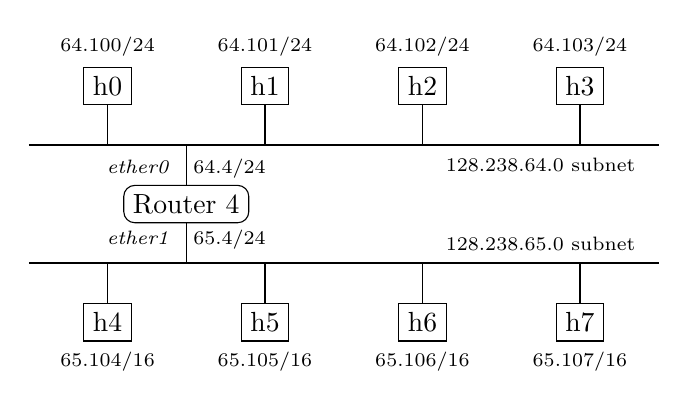
\begin{tikzpicture}
                \draw (0*2,3) node[draw,fill=white] (h0) {h0} -- +(0,-0.75) +(0,+0.5) node {\scriptsize 64.100/24};
                \draw (1*2,3) node[draw,fill=white] (h1) {h1} -- +(0,-0.75) +(0,+0.5) node {\scriptsize 64.101/24};
                \draw (2*2,3) node[draw,fill=white] (h2) {h2} -- +(0,-0.75) +(0,+0.5) node {\scriptsize 64.102/24};
                \draw (3*2,3) node[draw,fill=white] (h3) {h3} -- +(0,-0.75) +(0,+0.5) node {\scriptsize 64.103/24};
                \draw (0*2,0) node[draw,fill=white] (h4) {h4} -- +(0,+0.75) +(0,-0.5) node {\scriptsize 65.104/16};
                \draw (1*2,0) node[draw,fill=white] (h5) {h5} -- +(0,+0.75) +(0,-0.5) node {\scriptsize 65.105/16};
                \draw (2*2,0) node[draw,fill=white] (h6) {h6} -- +(0,+0.75) +(0,-0.5) node {\scriptsize 65.106/16};
                \draw (3*2,0) node[draw,fill=white] (h7) {h7} -- +(0,+0.75) +(0,-0.5) node {\scriptsize 65.107/16};
                \draw (0.5*2,1.5) node[draw,rounded corners,fill=white] (r4) {Router 4}
                    -- +(0,+0.75) +(0,+0.45) node {\scriptsize\textit{ether0}\quad 64.4/24}
                    -- +(0,-0.75) +(0,-0.45) node {\scriptsize\textit{ether1}\quad 65.4/24}
                ;
                \draw[thick] (-1,0.75) -- +({(3+1)*2},0);
                \draw[thick] (-1,2.25) -- +({(3+1)*2},0);
                \node at ({-1+(3+0.25)*2},2) {\scriptsize 128.238.64.0 subnet};
                \node at ({-1+(3+0.25)*2},1) {\scriptsize 128.238.65.0 subnet};
            \end{tikzpicture}
        \caption{Network configuration (Figure~2.9)}\label{fig:2.9}
    \end{figure}

Note: If you need the MAC address of the router interfaces, login to the router and run the following command in the router console. 

\fcolorbox{blue}{yellow!10}{ {R\textsubscript{4}\#} }
\lstset{backgroundcolor=\color{yellow!10}}
\begin{lstlisting}
	 show interfaces
\end{lstlisting}
    
    \begin{report}
        \item Explain the operation of proxy ARP.

        \item Why can a host in the 128.238.65.0 subnet reach a host in the 128.238.64.0 subnet, even though they have different subnet IDs?

        \item What are the \textbf{MAC} addresses corresponding to hosts in the 128.238.64.0 subnet, in the ARP table of a host in the 128.238.65.0 subnet?

        \item Give one advantage and one disadvantage of using proxy ARP.
    \end{report}

\section{** Gratuitous (Unsolicited) ARP}
    
    Start all devices and capture traffic of hosts \textit{h0} and \textit{h6} using wireshark

    \fcolorbox{blue}{lime!30}{ h\textsubscript{0}'s Wireshark} 
    \lstset{backgroundcolor=\color{lime!30}}
    \begin{lstlisting}
    Run wireshark on eth1 # or run tcpdump
    \end{lstlisting}

    \fcolorbox{blue}{lime!30}{ h\textsubscript{6}'s Wireshark} 
    \lstset{backgroundcolor=\color{lime!30}}
    \begin{lstlisting}
    Run wireshark on eth1 # or run tcpdump
    \end{lstlisting}
    
    Open the console of host \textit{h7}, you can send the gratuitous ARP manually by use the following command 
    
    \fcolorbox{blue}{red!10}{ {h\textsubscript{7}}'s Console }
    \lstset{backgroundcolor=\color{red!10}}
    \begin{lstlisting}
    arping -c 4 -A -I eth1 128.238.65.106
    \end{lstlisting}
    
    see ARP Table of host \textit{h6} by using the following command
    
    \fcolorbox{blue}{red!10}{ {h\textsubscript{6}}'s Console }
    \lstset{backgroundcolor=\color{red!10}}
    \begin{lstlisting}
    arp -a
    \end{lstlisting}
    
    Now reboot host \textit{h7} using the following command again
    
    \fcolorbox{blue}{red!10}{ {h\textsubscript{7}}'s Console }
    \begin{lstlisting}[emph={eth1,h7-ip,h6-ip}]
    arping -c 4 -A -I eth1 128.238.65.106
    \end{lstlisting}
    
    \fcolorbox{blue}{red!10}{ {h\textsubscript{6}}'s Console }
    \lstset{backgroundcolor=\color{red!10}}
    \begin{lstlisting}
    arp -a
    \end{lstlisting}
    
    print the gratuitous ARP request for your lab report.
    
    \begin{report}
        \item What is the purpose of gratuitous ARP?
    
        \item List the sender IP address, target IP address, sender \textbf{MAC} address, and target \textbf{MAC} address of the gratuitous ARP you saved.

        \item What is the ARP table in \textit{h5}?
    \end{report}


\part{Exercise with ICMP and \texttt{ping}}\label{sec:icmp-ping}
    The following exercises use the previous network topology shown in \hyperref[fig:2.9]{Figure~2.9}.

\section{ping ICMP}
    While \lstinline{wireshark} is running to capture traffic from your machine,
    
    \fcolorbox{blue}{lime!30}{ {h\textsubscript{0}}'s Wireshark }
    \lstset{backgroundcolor=\color{lime!30}}
    \begin{lstlisting}[emph={remote-host}]
    Run wireshark on eth1, Filter: ip.addr == 128.238.64.100 && ip.addr == remote-host
    \end{lstlisting}
    
     Execute this command to test whether the remote host is reachable.
    
    \fcolorbox{blue}{red!10}{ {h\textsubscript{0}}'s Console }
    \lstset{backgroundcolor=\color{red!10}}
    \begin{lstlisting}[emph={remote-host}]
    ping -sv remote-host
    \end{lstlisting}
   
   (remote-hast can be \textit{h1}, \textit{h4} or \textit{h5} IP address)
    
    Save the \lstinline{wireshark} and \lstinline{ping} outputs for the future study on \lstinline{ping}.
    
    \begin{report}
        \item What ICMP messages are used by \lstinline{ping}?
    \end{report}

\section{ICMP Port Unreachable}
    While \lstinline{wireshark} is running to capture traffic from your machine,
    
    \fcolorbox{blue}{lime!30}{ {h\textsubscript{0}}'s Wireshark }
    \lstset{backgroundcolor=\color{lime!30}}
    \begin{lstlisting}[emph={remote-host}]
    Run wireshark on eth1, Filter: ip.addr == 128.238.64.100 && ip.addr == remote-host
    \end{lstlisting}
    
 execute the following \lstinline{socket} command to send a UDP datagram to the remote host

    \fcolorbox{blue}{red!10}{ {h\textsubscript{0}}'s Console }
    \lstset{backgroundcolor=\color{red!10}}
    \begin{lstlisting}[emph={remote-host}]
    socket -i -u -n1 -w1000 remote-host 88888
    \end{lstlisting}
(remote-host can be \textit{h1}, \textit{h4} or \textit{h5} IP address)

    Save the \lstinline{wireshark} output for the lab report.

    \begin{report}
        \item Study the saved ICMP port unreachable error message (See \hyperref[fig:2.7]{Figure~2.7} of the reference book.).
            Why are the first 8 bytes of the original IP datagram payload included in the ICMP message?
    \end{report}

\section{ICMP Network Unreachable}
   While running \lstinline{wireshark} for host \textit{h2} to capture ICMP messages,
    
    \fcolorbox{blue}{lime!30}{ {h\textsubscript{2}}'s Wireshark }
    \lstset{backgroundcolor=\color{lime!30}}
    \begin{lstlisting}
    Run wireshark on eth1
    \end{lstlisting}
    
     \lstinline{ping} a host with IP address \lstinline{128.238.60.100} by use the following command
    
    \fcolorbox{blue}{red!10}{ {h\textsubscript{2}}'s Console }
    \lstset{backgroundcolor=\color{red!10}}
    \begin{lstlisting}
    ping 128.238.60.100
    \end{lstlisting}
    
    and Save the \lstinline{ping} output.
    
    \begin{report}
        \item Can you see any traffic sent on the network? Why? Explain what happened from the \lstinline{ping} output.

        \item List the different ICMP messages you captured in \nameref{sec:icmp-ping}.
            Give the values of the type and code fields.
    \end{report}

\part{Exercises with IP address and subnet mask}
    In this section, we will observe what happens when the same IP address is assigned to two different hosts.
    We will also set an incorrect subnet mask for hosts and see what are the consequences.
    For the next two exercises, we use only four host from single segment network (\hyperref[fig:1.3]{Figure~1.3}).

\section{Duplicate IP}\label{sec:duplicate-ip}
    Change the IP address of your hosts as shown in \hyperref[tab:2.3]{Table~2.3}.

    \begin{table}[H]
        \caption{Host IP addresses and network masks for \nameref{sec:duplicate-ip} (Table~2.3)}\label{tab:2.3}
        \centering
        \begin{tabular}{ c c c c }
            \hline \hline
            Host & IP Address & Subnet Mask \\
            \hline 
            h0 & 128.238.66.100 & 255.255.255.0 \\
            h1 & 128.238.66.100 & 255.255.255.0 \\
            h2 & 128.238.66.102 & 255.255.255.0 \\
            h3 & 128.238.66.103 & 255.255.255.0 \\
            \hline \hline
            \end{tabular}
    \end{table}
Delete the entries for all hosts other than your host from ARP table.
\begin{itemize}
	\item Start devices \textit{h0, h1, h2, h3} by right-clicking on them and selecting \texttt{start}.
	\item Open host \textit{h1}'s console and change IP address of it by running the following commands.
\end{itemize}
       \fcolorbox{blue}{green!10}{ {h\textsubscript{1}}'s Console }
        \lstset{backgroundcolor=\color{green!10}}
        \begin{lstlisting}
        ip address del 128.238.66.101/24 dev eth1
        ifconfig eth1 128.238.66.100 netmask 255.255.255.0       
    \end{lstlisting}

Run \lstinline{wireshark} for all the hosts. 

 \fcolorbox{blue}{lime!30}{ {h\textsubscript{0}}, {h\textsubscript{1}}, {h\textsubscript{2}} and {h\textsubscript{3}}'s Wireshark }
\lstset{backgroundcolor=\color{lime!30}}
\begin{lstlisting}
    Run Wireshark on eth1
\end{lstlisting}
Now, do the following three experiments:
    \begin{enumerate}
        \item Execute \lstinline{telnet} from one of two hosts with the duplicate IP address to a host with unique IP address by run following commands(e.g.\ \textit{h0} $\rightarrow$ \textit{h2}).
        
        \fcolorbox{blue}{red!10}{ {h\textsubscript{0}}'s Console }
        \lstset{backgroundcolor=\color{red!10}}
        \begin{lstlisting}
        telnet 128.238.66.102
        \end{lstlisting}
        
        Now, from the other host with the duplicate IP address, execute \lstinline{telnet} command to the same host by run following command(\textit{h1} $\rightarrow$ \textit{h2}).
        
        \fcolorbox{blue}{red!10}{ {h\textsubscript{1}}'s Console }
        \lstset{backgroundcolor=\color{red!10}}
        \begin{lstlisting}
        telnet 128.238.66.102
        \end{lstlisting}
        
        \fcolorbox{blue}{red!10}{ {h\textsubscript{0}},  {h\textsubscript{1}} and  {h\textsubscript{2}}'s Console }
        \lstset{backgroundcolor=\color{red!10}}
        \begin{lstlisting}
        arp -a
        \end{lstlisting}
        
        Observe what happens and save the \lstinline{wireshark} output and the ARP tables in all the hosts in your group.
        
        \item Execute the following commands
        
        \fcolorbox{blue}{red!10}{ {h\textsubscript{2}}'s Console }
        \lstset{backgroundcolor=\color{red!10}}
        \begin{lstlisting}
        telnet 128.238.66.100
        \end{lstlisting}
        
        Which host provides the telnet connection? Why?
        
        \item Execute the following command 
        
        \fcolorbox{blue}{red!10}{ {h\textsubscript{3}}'s Console }
        \lstset{backgroundcolor=\color{red!10}}
        \begin{lstlisting}
        telnet 128.238.66.100
        \end{lstlisting}
 
         Which host is connected to \textit{h3}? Why?
    \end{enumerate}
    
    \begin{report}
        \item Explain what happened in the first case and why.
            Answer the questions for the second and third cases.
    \end{report}

\section{IP Subnets}\label{sec:ip-subnets}
    Change the host IP addresses and the subnet masks as shown in \hyperref[tab:2.4]{Table~2.4}.
    Note that two hosts in each group (\textit{h0} and \textit{h3}) are assigned an incorrect subnet mask.

    \begin{table}[H]
        \caption{Host IP addresses and network masks for \nameref{sec:ip-subnets} (Table~2.4)}\label{tab:2.4}
        \centering
        \begin{tabular}{ c c c }
            \hline \hline
            Host & IP Address & \makebox[7.3em][c]{Subnet Mask} \\
            \hline 
            h0 & 128.238.66.100 & \makebox[7.3em][l]{255.255.255.240} \\
            h1 & 128.238.66.101 & \makebox[7.3em][l]{255.255.255.0} \\
            h2 & 128.238.66.102 & \makebox[7.3em][l]{255.255.255.0} \\
            h3 & 128.238.66.120 & \makebox[7.3em][l]{255.255.255.240} \\
            \hline \hline
            \end{tabular}
    \end{table}
\begin{itemize}
	\item Start hosts \textit{h0, h1, h2, h3} by right-clicking on them and selecting \texttt{start}.
	\item Open host \textit{h0}'s console and change its IP address by running the following commands
    
    \fcolorbox{blue}{green!10}{ {h\textsubscript{0}}'s Console }
    \lstset{backgroundcolor=\color{green!10}}
        \begin{lstlisting}
        ip address del 128.238.66.100/24 dev eth1
        ifconfig eth1 128.238.66.100 netmask 255.255.255.240
        \end{lstlisting}
(note: you can used  \lstinline{ip address add 128.238.66.100/28 dev eth1} command instead of \\\lstinline{ifconfig eth1 128.238.66.100 netmask 255.255.255.240} )
    
  	\item Open host \textit{h3}'s Console and change its IP address by running the following command   
  	 
    \fcolorbox{blue}{green!10}{ {h\textsubscript{3}}'s Console }
        \lstset{backgroundcolor=\color{green!10}}
        \begin{lstlisting}
        ip address del 128.238.66.103/24 dev eth1
        ip address add 128.238.66.120/28 dev eth1
    \end{lstlisting}
\end{itemize}
    
    Using \lstinline{wireshark}, capture the packets for the following cases: 
    
     \fcolorbox{blue}{lime!30}{ {h\textsubscript{0}}, {h\textsubscript{1}} and {h\textsubscript{3}}'s Wireshark }
    \lstset{backgroundcolor=\color{lime!30}}
    \begin{lstlisting}
    Run wireshark on eth1
    \end{lstlisting}
    
    \begin{enumerate}
        \item When \textit{h0} \lstinline{ping}s one of the hosts that have the correct subnet mask.(Used the following command)
        
        \fcolorbox{blue}{red!10}{ {h\textsubscript{0}}'s Console }
        \lstset{backgroundcolor=\color{red!10}}
        \begin{lstlisting}
        ping 128.238.66.101
        \end{lstlisting}
        
        \item When \textit{h3} \lstinline{ping}s one of the hosts that have the correct subnet mask. (Used the following command)
        
        \fcolorbox{blue}{red!10}{ {h\textsubscript{3}}'s Console }
        \lstset{backgroundcolor=\color{red!10}}
        \begin{lstlisting}
        ping 128.238.66.101
        \end{lstlisting}
        
               \item When a host with the correct subnet mask \lstinline{ping}s \textit{h0}. (Used the following command)
        
        \fcolorbox{blue}{red!10}{ {h\textsubscript{1}}'s Console }
        \lstset{backgroundcolor=\color{red!10}}
        \begin{lstlisting}
        ping 128.238.66.100
        \end{lstlisting}
        
        \item When a host with the correct subnet mask \lstinline{ping}s \textit{h3}. (Used the following command)

        \fcolorbox{blue}{red!10}{ {h\textsubscript{1}}'s Console }
        \lstset{backgroundcolor=\color{red!10}}
        \begin{lstlisting}
        ping 128.238.66.120
        \end{lstlisting}
        
    \end{enumerate}
    
    \begin{report}
        \item Explain what happened in each case according to the saved \lstinline{wireshark} outputs.
            Explain why \textit{h3} could not be reached from other hosts, whereas \textit{h0}, which has the same incorrect subnet mask, could communicate with the other hosts.
    \end{report}
\end{document}